\documentclass[english,  % Standardmäßig deutsche Eigenarten, englisch -> english
parskip=full,   % Absätze durch Leerzeile trennen
%bibliography=totoc,  % Literatur im Inhaltsverzeichnis (ist unüblich)
%draft,  % TODO: Entwurfsmodus -> entfernen für endgültige Version
headsepline]{scrartcl}

\usepackage[a4paper,left=3.5cm, right=3.5cm,top=3.5cm, bottom=5.7cm]{geometry}
\usepackage[utf8]{inputenc}  % Kodierung der Datei
\usepackage[T1]{fontenc}  % Vollen Umfang der Schriftzeichen
\usepackage[english]{babel}  % Sprache auf Deutsch (neue Rechtschreibung)
\usepackage{booktabs}
\usepackage{float}
% Mathematik und Größen
\usepackage{amsmath}
\usepackage[locale=DE,  % deutsche Eigenarten, englisch -> EN
separate-uncertainty,  % Unsicherheiten seperat angeben (mit ±)
]{siunitx}
%http://texdoc.net/texmf-dist/doc/latex/siunitx/siunitx.pdf
\usepackage{physics}  % Erstellung von Gleichungen vereinfachen
\usepackage{svg}    
\usepackage{graphicx}  % Bilder einbinden \includegraphics{Pfad/zur/Datei(ohne Dateiendung)}
\usepackage[
backend=biber,
style=nature,
sorting=ynt
]{biblatex}
\usepackage{wrapfig}
\usepackage[version=4,arrows=pgf]{mhchem}  % Chemie Paket für Isotopenschreibweise etc.
\usepackage{wrapfig}
\usepackage{floatflt}
\usepackage{enumerate}
% Gestaltung
%\usepackage{microtype}  % Mikrotypographie (kann man am Ende verwenden)
\usepackage{booktabs}  % schönere Tabellen
%\usepackage[toc]{multitoc}  % mehrspaltiges Inhaltsverzeichnis
\usepackage{multicol}
\usepackage{csquotes}  % Anführungszeichen mit \enquote
\usepackage{caption}  % Anpassung der Bildunterschriften, Tabellenüberschriften
\usepackage{subcaption}  % Unterabbildungen, Untertabellen, …
\usepackage{cprotect}
\usepackage{enumitem}  % Listen anpassen
\usepackage{siunitx}
\usepackage{eufrak}
%Feynman-Diagramme package
\usepackage{tikz-feynman}

\usepackage{dirtytalk}
\usepackage{subcaption}
\usepackage{textcomp}
\usepackage[hidelinks]{hyperref}  % Links und weitere PDF-Features
\usepackage{hyperref}
\usepackage[]{cleveref} %noabbrev für ausgeschriebene verweise

\setlist{itemsep=-10pt}  % Abstände zwischen Listenpunkten verringern
\addbibresource{bibliography.bib}
% Manipulation des Seitenstils
\usepackage{scrlayer-scrpage}
% Kopf-/Fußzeilen setzen
\pagestyle{scrheadings}  % Stil für die Seite setzen
\clearscrheadings  % Stil zurücksetzen, um ihn neu zu definieren
\automark{section}  % Abschnittsnamen als Seitenbeschriftung verwenden
\ofoot{\pagemark}  % Seitenzahl außen in Fußzeile
\ihead{\headmark}  % Seitenbeschriftung mittig in Kopfzeile
%\setkomafont{\headsepline}{}
\setcounter{tocdepth}{2} %set depth of printed table of contets.
\makeatletter

%\renewcommand\tableofcontents{% Absatz vor Gliederungspunkten
   % \begin{multicols}{2}[\section*{\contentsname
 %       \@mkboth{%
  %         \MakeUppercase\contentsname}{\MakeUppercase\contentsname}}]%
 %   \@starttoc{toc}%
 %   \end{multicols}%
 %   }

\makeatother %print dots in sections in toc.
\hypersetup{
    colorlinks=true,
    linkcolor=blue,
    citecolor=red,
    filecolor=magenta,      
    urlcolor=cyan,
    pdftitle={Overleaf Example},
    pdfpagemode=FullScreen,
    }

% TODO: Titel und Autor, … festlegen
\newcommand*{\titel}{Lifetime of Muons}
\newcommand*{\autor}{Lukas König, Steven Gebel}
\newcommand*{\abk}{}
\newcommand*{\betreuer}{Nab Abhishek}
\newcommand*{\messung}{19. November 2021}
\newcommand*{\ort}{ASB/K15 a}
\newcommand{\diff}[1]{\frac{\mathrm{d}}{\mathrm{d}#1}}
\newcommand{\mus}{\,\si{\mu s\:}}
\newcommand{\ten}[1]{\cdot10^{#1}}
\newcommand{\dsys}{\Delta_\text{sys}}
\newcommand{\logdiff}[1]{\left(\frac{\Delta #1}{#1}\right)^2}
\newcommand{\dunderline}[1]{\underline{\underline{#1}}}
\newcommand{\bcref}[1]{\namecref{#1} \textcolor{blue}{\labelcref{#1}}}
\newcommand{\e}{\mathrm{e}}
\hypersetup{pdfauthor={\autor}, pdftitle={\titel}}  % PDF-Metadaten setzen

% automatischen Titel konfigurieren
\titlehead{Fortgeschrittenenpraktikum LM \abk \hfill Technische Universität Dresden}
\subject{Lab report}
\title{\titel}
\author{\autor}
\date{\begin{tabular}{ll}
Protocol: & \today\\
Measurement: & \messung\\
Place: & \ort\\
Supervisor: & \betreuer\end{tabular}}
\begin{document}
\begin{titlepage}
\maketitle  % Titel setzen
\tableofcontents  % Inhaltsverzeichnis setzen
\end{titlepage}
\section{Introduction}
\subsection{Task}
Calculate the Fermi coupling constant $G_F$ and vacuum expectation value, $v$, of the BEH Field from the measured lifetime, along with the error propagation to find the uncertainty in the calculated value. Compare the calculated values with the literature values.

\subsection{Theoretical background}
In this experiment the mean lifetime of muons is measured. Those muons are a result of high energy protons from cosmic radiation, that decay into pions after collisions with earth's atmospheres atomic nuclei. The simplest reactions are:
\begin{align*}
    p+p \rightarrow& \,p+n+\pi^+\\
    p+n \rightarrow& \,p+p+\pi^-
\end{align*}
The charged pions $\pi^+$ and $\pi^-$ decay to 100\% through the weak interaction:
\begin{align*}
    \pi^+ \rightarrow& \, \mu^+ +\nu_{\mu}\\
    \pi^- \rightarrow& \, \mu^- +\nu_{\bar{\mu}}
\end{align*}
Now the negative/positively charged muon decays with a mean lifetime of \\$\tau_{\mu} = (2.19703 \pm 0.00004)\cdot 10^{-6}\si{\second}$ \cite{Zyla:2020zbs} according to:
\begin{align*}
    \mu^+ \rightarrow& \, e^+ + \nu_e + \bar{\nu}_{\mu}\\
    \mu^- \rightarrow& \, e^- + \bar{\nu}_e + \nu_{\mu}\\
\end{align*}
The muons are able to reach earth's surface, since they move with relativistic velocities and thus time dilatation and length contraction play a role.\\
Thus, by determining the lifetime of muons one can calculate the coupling constant of the weak interaction, while $\mu^+$ and $\mu^-$ have roughly the same lifetime:
\begin{equation}
\label{eq:fermi}
    \tau_{\mu}^{-1} = G_F^2\cdot \frac{m_{\mu}^5}{192\pi^3}
\end{equation}
From the obtained Fermi constant $G_F$ one can calculate the vacuum expectation value of the \textsc{Brout-Engert-Higgs}-field $v$, without explaining further how to obtain this relation, since this would go beyond this quick overview of the theoretical background. In short, for the $\mu$-decay two variants of Feynman amplitudes $\mathfrak{M}$ can be calculated. One by describing it via the Fermi four-point interaction which results in $\mathcal{M}_F\propto \sqrt{2}G_F$ and via the standard model process (considering gauge bosons which is the more proper way): $\mathcal{M}_W\propto\frac{g_w^2g_{\mu\nu}}{4m^2_w}$. Now setting those Fermi amplitudes equal and considering that the gauge boson masses $m_W$ are related to the vacuum expectation value of the \textsc{Brout-Engert-Higgs}-field and weak coupling constant $g_w$ via $m_w=\frac{v\cdot g_w}{2}$ one ends up with:
\begin{equation}
   \sqrt{2}\cdot G_F = \frac{1}{v^2}
   \label{eq:higgs}
\end{equation}
\subsection{Measurement setup}
\subsubsection{Used gear}
    \begin{itemize}
        \item Tektronix TDS 2014 Oscilloscope
        \item control unit
    \end{itemize}
\subsubsection{Preliminary measurement}
The measurement setup for the preliminary setup
consists of a block of plastic scintillators as depicted in \cref{fig:setup2} with photomultipliers mounted at each end and connected to the scintillators via a soft plastic material.\\
The output signals are sent to a discriminator with adjustable threshold of $\SI{100}{\milli \volt}$.\\
The resulting signals $\mathfrak{1}$ and $\mathfrak{2}$ are sent to a coincidence unit. The coincidence signal $\mathfrak{12}$ indicates that a particle of cosmic radiation has passed through or has been stopped or that particles from other events have been stopped.\\
These coincidence signals start the TDC and if the muon decays within $\SI{10}{ms}$ a coincidence $(\mathfrak{12})_{delay}$ is used as a stop of the TDC. Finally the sum of all delayed coincidences leads to the lifetime of $\mu^+$ and $\mu^-$.

\begin{figure}[H]
    \centering
    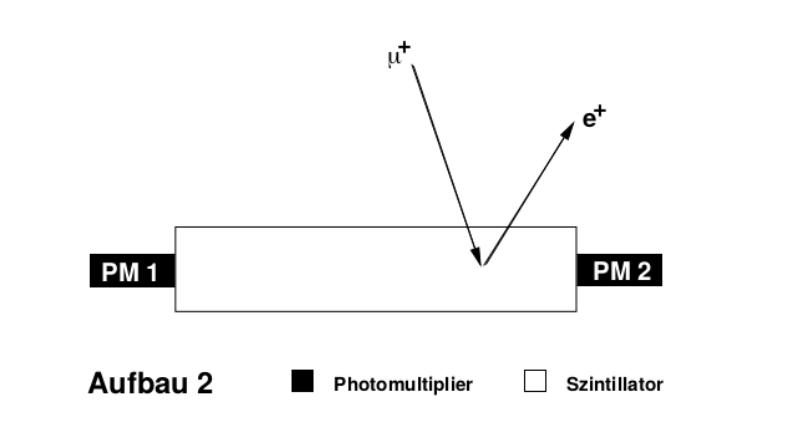
\includegraphics[width=0.6\linewidth]{setup2.png}
    \caption{Measurement setup for the preliminary setup \cite{anleitung}.}
    \label{fig:setup2}
\end{figure}
\subsubsection{Main measurement}
The experimental setup for the long term  main measurement consists of two copper plates of thickness $\SI{1}{\cm}$ and two scintillators above and one below the copper plates. The scintillating light is read out by photomultiplier tubes (PM) which is descreibed in more detail in the following section.\\
A moun stopped in the copper target is indicated by signal $\mathfrak{12\bar{3}}$ meaning detector $\mathfrak{1}$ and $\mathfrak{2}$ respond but not detector $\mathfrak{3}$. This creates a start signal for timing in a Time-to-Digital Converter (TDC). For the TDC to stop, a signal $\mathfrak{2\bar{3}}$ for the upward-emitted $e^+$ and $\mathfrak{\bar{2}3}$ for the downward-emitted $e^+$ as shown in \cref{fig:setup}.\\
Since the start signal in the TDC opens a time window of $\SI{10}{\mus}$ for the stop signal, accidental coincidences (e.g. low-energy content of cosmic radiation) are considerably reduced.\\
The PM's signals are converted by a discriminator into uniformly shaped signals with an output width of $\SI{40}{\nano \second}$. The discriminator also suppresses noise (low signal levels $>\SI{-100}{\milli \volt}$ since the electronic pulse is negative).\\
All the events are read out by the PC and stored to disk.
\begin{figure}[H]
    \centering
    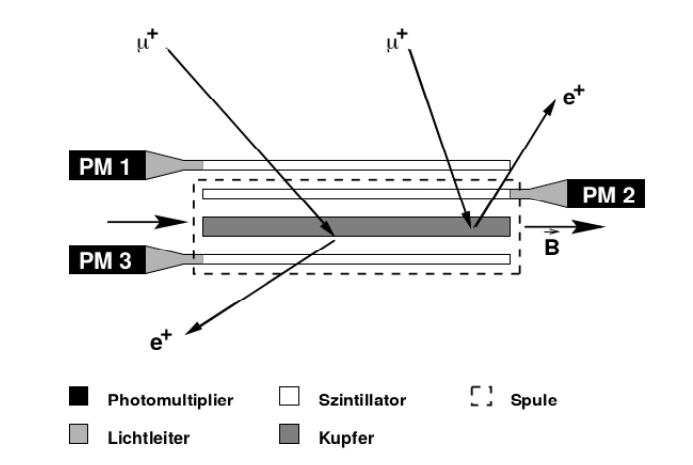
\includegraphics[width=0.6\linewidth]{setup.png}
    \caption{Measurement setup for the long-term measurement. \cite{anleitung}}
    \label{fig:setup}
\end{figure}
\subsubsection{Scintillator}
Ionizing radiation that enters the scintillators anorganic or organic material (in this experiment mostly muons, electrons and positrons) creates electron-hole-pairs which excite so called activators, resulting in the emission of photons. These photons have a wavelength in the range of visible light. In this experiment, organic(plastic)-scintillators are used in which fluorescent molecules (activators) can be stimulated which then emit photons in the UV-spectrum.
\subsubsection{Photomultiplier}
The emitted photons from the scintillator then hit a photodiode that transforms the photons via the photoelectric effect in electrical signals, depending on the amount of photons, the signal can consist of just a few electrons. In order to measure even such small signals, it is strengthened in a secundary electron multiplier. In this multiplier a high voltage is applied so that all electrons flow in one direction. On their way to the anode the electrons hit dynodes resulting in the creation of more and more free electrons in exponential growth. The electron count that is measured in the end depends on the initial amount of photons and on the high voltage, that is why it is important to set the voltage carefully.

\subsection{Statistical analysis}
To estimate the parameter $\tau$ from the given channel data, the maximum-likelihood-method will be employed. For this method, the PDF $P(\Vec{N}|\tau)$ of the data (in this case the event count for a given time interval) has to be known. The likelihood-function $L(\tau|N_1, \dots, N_K)$ is then given as
\[
L(\tau|N_1, \dots, N_K)=\prod_{i=1}^KP(N_i|\tau).
\]
It represents the probability of measuring the given data as a function of the parameter $\tau$. The best value for $\tau$ is then that, which maximizes $L$. In practice, it is easier to work with the logarithm of $L$ (turning the multiplication into summation), and so the following equation
\[
\diff{\tau}\ln L\left. \right|_{\tau=\hat{\tau}}=0\label{eq:Lcond}
\]
has to be satisifed.
\subsubsection{Usage for exponential decay law}
The PDF is here given as 
\[
P(t_i|\tau)=\frac{1}{\tau}\e^{-t_i/\tau}
\]
This is however only normed for an infinitely long measurement, so to account for this, in reality the modified PDF
\[
P(t_i|\tau)=\frac{1}{\tau}\e^{-t_i/\tau}\frac{1}{1-\e^{-T/\tau}}
\]
has to be used. From this, the logarithm of the likelihood-function is calculated to be 
\[
\ln L=\sum\left(-\frac{t_i}{\tau}-\ln\tau-\ln\left(1-\e^{-T/\tau}\right)\right)\label{eq:Lexp}
\]
To satisfy \cref{eq:Lcond}, one now finds:
\begin{align}
\diff{\tau}\ln L\left. \right|_{\tau=\hat{\tau}}&=\sum\left(\frac{t_i}{\tau^2}-\frac{1}{\tau}+\frac{1}{\tau^2}\frac{T\e^{-T/\tau}}{1-\e^{-T/\tau}}\right)\overset{!}{=}0\\
\Rightarrow\hat{\tau}&=\frac{1}{N}\sum t_i+\frac{T\e^{-T/\tau}}{1-\e^{-T/\tau}}
\end{align}
This transcendental equation now has to be solved numerically. In the case of this experiment, $N_i$s are measured in $i$ time-intervals. $\sum t_i$ is thus replaced by $\dfrac{1}{N}\sum N_k\cdot t_k$, where $N$ is the total number of counts and $t_k$ the estimated average decay time in the channel, which is in a good approximation the channel-center. The error-calculation will be explained in detail in \cref{sec:evalexp}.
\subsubsection{Application to Poisson-distribution}
The probability to observe $N$ events when $f$ events are expected is described (in this experiment) by a Poisson-distribution. For a fixed $\tau$, the probability of measuring $N_i$ events in channel $i$ while expecting $f_i$ events is given by
\[
P(N_i|f_i)=\dfrac{f_i^{N_i}\cdot\e^{-f_i}}{N_i!}
\]
The standard deviation of the Poisson-distribution for the observed $N_i$ around its mean value $f_i$ is
\[
\sigma_i=\sqrt{f_i}
\]
We now consider bins of times $t_i, t_i+\Delta t$. $f_i$ now depends on the position and width of the channel, the parameter $\tau$ and the normalization $N_0$ of the exponential function $f_i=\dfrac{N_0}{\tau}\e^{-t_i/\tau}$. With $N$ events and $K$ bins, the following applies:
\begin{align}
    f_i&=\int_{t=t_i}^{t=t_i+\Delta t}\dfrac{N_0}{\tau}\e^{-t_i/\tau}\dd t\approx f_i\approx\frac{N_0}{\tau}\e^{-(t_i+\Delta t/2)/\tau}\cdot\Delta t, \\
N_0&=\frac{N}{\e^{t_1/\tau}-\e^{-(t_K+\Delta t)/\tau}},\\
\text{and }N&=\int_{t=t_1}^{t_K+\Delta t}\dfrac{N_0}{\tau}\e^{-t_i/\tau}\dd t
\end{align}
If one minimizes $-2\ln L$ instead of maximizing $L$, one can obtain the standard deviation: a deviation of one $\sigma_\hat{\tau}$ leads to a increase of one unit of $-2\ln L$ compared to the minimum \cite{stats}.
The value of $-2\ln L$ results %welches missing }???
\begin{align}
    -2\ln L&=-2\sum_iN_i\ln f_i+2\sum_if_i+2\sum_i\ln(N_i!)\\
    &=-2\sum_iN_i\ln f_i+2N+2\sum_i\ln(N_i!)
\end{align}
$2N+2\sum_i\ln(N_i!)$ is independent of $\tau$, so it is sufficient to minimize
\[
-2\sum_iN_i\ln f_i.
\]
This minimum has to be found numerically.
\subsubsection{Application to Gauss-distribution}
in the limiting case of large values, the Gauss-distribution results from the Poisson-distribution ($f>10$). The PDF is
\[
P(N_i|\tau)=\dfrac{1}{\sqrt{2\pi\sigma_i^2}}\exp{-\dfrac{(N_i-f_i)^2}{2\sigma_i^2}},
\]
where $f_i$ and $N_0$ are defined as above, and
\[\sigma_i=\sigma(f_i)=\sqrt{f_i}\approx\sqrt{N_i}\label{eq:approx}.\] One proceeds as with the Poisson distribution and gets:
\[
-2\ln L = \sum_i\ln(2\pi\sigma_i^2)+\sum_i\frac{N_i-f_i)^2}{\sigma_i^2}
\]
$\sum_i\ln(2\pi\sigma_i^2)$ is, following the approximation \cref{eq:approx} independent of $\tau$, therefore only
\[
\chi^2=\sum_i\frac{(N_i-f_i)^2}{\sigma_i^2}
\]
has to be minimized. This is called $\chi^2$-method. This function should follow the $\chi^2$-distribution for Gaussian  distributed random variables, which can be checked with a table. 
\section{Procedure}\label{Procedure}
\subsection{Preliminary Test}
\subsubsection{Recording the characteristic $U_{PM1}-U_{PM2}$ calibration curve}
In order to record the calibration points, the LED is connected to the Pulse Generator, as well as the outputs to the oscilloscope, with the frequency at approx $1\si{k\hertz}$.\\
Now $U_{PM1}$ is altered from $1700 \si{volt}$ to $2350\si{\volt}$ in $50\si{\volt}$ steps while adjusting $U_{PM2}$ stepwise, so that the amplitudes of the two pulses on the oscilloscope are approximately the same.
\begin{figure}[H]
    \centering
    \includesvg[width=0.5\linewidth]{vorversuch1.svg}
    \caption{Visualized data for the calibration curve with the linear fit function in green.}
    \label{fig:vorversuch1}
\end{figure}
For the subsequent use, the data is fitted to a linear function via\\ \verb+scipy.optimize.curve_fit+, while taking the measurement uncertainty in $U_{PM2}$ from the oscillator coming from the differing resolutions into consideration.\\
One ends up with a nicely visible linear $U_{PM2}(U_{PM1})$-relation and the fit parameters, while the measurement uncertainties are interpreted as statistical and result from the covariance-matrix of \verb+curve_fit+ as in all further fits:
\begin{align*}
\text{A} \pm \Delta \text{A}=&(0.79\pm0.01)\\
\text{B} \pm \Delta \text{B}=&(307\pm12)\si{\volt}
\end{align*}
The last 2 measurement points were neglected for the linear fit, since they do clearly not obey to a linear function in contrast to the previous data points while it is also clear, that for $U_{PM1} \ge \SI{2100}{\volt}$ the data tends to differ more and more from the linear fit.

\begin{table}[H]
    \centering
    \caption{Data for the first preliminary measurement. The measurement uncertainty $\Delta$U holds for both voltages, since they were adjusted on the same oscilloscope.}
    \begin{tabular}{c|c|c}
         $U_{PM1} / \si{\volt}$&$U_{PM2} / \si{\volt}$& $\Delta U / \si{\volt}$ \\ \hline \hline
         1700&1657&1\\
         1750&1710&1\\
         1800&1755&2.5\\
         1850&1799&2.5\\
         1900&1835&5\\
         1950&1878&5\\
         2000&1908&5\\
         2051&1942&5\\
         2099&1974&5\\
         2150&1997&10\\
         2200&2016&10\\
         2251&2024&10\\
         2301&2037&10\\
         2350&2039&10\\
    \end{tabular}
    \label{tab:vv1}
\end{table}

\subsubsection{Equal amplitude coincidence measurement}
For this preliminary measurement, the coincidence signal (12) is placed on a channel of the counting unit
In order to guarantee that the relative error $\frac{\Delta Z_{12}}{Z_{12}} \le 1\%$ for $U_{PM1}=\SI{2000}{\volt}$, the measurement time is increased until one reaches $t=\SI{435}{\second}$ since the experimentators captured $\ge 10000$ events in this time, while taking into consideration, that the error is calculated by $\Delta Z_{12}=\sqrt{Z_{12}}$ (Poisson statistics for decays) and thus this amount of events is needed for good statistics. These errors can be visible as errorbars in \cref{fig:vorversuch2}. \\\\
\begin{figure}[H]
    \centering
    \includesvg[width=0.5\linewidth]{vorversuch2.svg}
    \caption{Visualized data for the equal amplitude coincidence measurement with coloured areas of behaviour of the counts $Z_{12}$.}
    \label{fig:vorversuch2}
\end{figure}
Having obtained the right measurement time, one draws on the $U_{PM2}(U_{PM1})$-relation in order to set $U_{PM2}$ while $U_{PM1}$ is altered in the range of $\SI{1750}{\volt}$ to $\SI{2200}{\volt}$ in $\SI{50}{\volt}$ increments and two extra measurement points in the saturation area (green in \cref{fig:vorversuch2}) between $\SI{1900}{\volt}\le U_{PM1} \le \SI{2000}{\volt}$.\\
In \cref{fig:vorversuch2} three phases are visible and colored: 
\begin{enumerate}
    \item red captures the linear part of the counts, meaning that for higher voltages, more muon coincidences are detected.
    \item in the green area, a saturation point at $ U_{PM1} \approx \SI{1950}{\volt}$ is visible for the muons.
    \item for voltages $U_{PM1} \ge \SI{2000}{\volt}$ (blue area) the coincidence rate grows $\propto \exp(U_{PM1})$.
    The data proves this assumption, since it can be fitted to an exponential function (see fit in \cref{fig:vorversuch2}).
    This means, that for those values of $U_{PM1}$ one increasingly counts different events (noise) apart from muons and consequently, one does use $U_{PM1} \approx \SI{2000}{\volt}$ as the working voltage.
\end{enumerate}

\begin{table}[H]
    \caption{Measurement data for the second preliminary measurement.}
    \centering
    \begin{tabular}{c|c|c|c}
    $U_{PM1}/\si{\volt}$&$U_{PM2}/\si{\volt}$&  $Z_{12}$& $\Delta Z_{12}$\\ \hline \hline
    1750&1705&1280&36\\
    1800&1745&2718&52\\
    1850&1785&4634&68\\
    1900&1825&6583&81\\
    1925&1845& 7101&84\\
    1950&1865& 8415&92\\
    1975&1885& 9100&95\\
    2000&1905& 10017&100\\
    2050&1945& 13250&15\\
    2100&1984& 17919&134\\
    2150&2024& 26795&164\\
    2200&2064& 42167&205
    \end{tabular}
    \label{tab:vv2}
\end{table}
The fit parameters for the linear fit are given by:
\begin{align*}
\text{A} \pm \Delta \text{A}=& (32.6\pm0.7)\si{\per \volt}\\
\text{B} \pm \Delta \text{B}=& (-55780 \pm1289)
\end{align*}
And for the exponential fit, while the statistical measurement uncertainties given by \verb+curve_fit+ are too big given the fact, that there just a few data points to fit to, resulting in:
\begin{equation}
\text{A} = \SI{139}{\volt}, \,\,\, \text{B} = \SI{5885}{\volt}, \,\,\, \text{C} = \SI{1680}{\volt}, \,\,\, \text{D} = \SI{0.011}{\per\volt}
\end{equation}
\clearpage
\section{Evaluation}
\subsection{Main experiment}
\begin{floatingfigure}{0.5\linewidth}
    \centering
    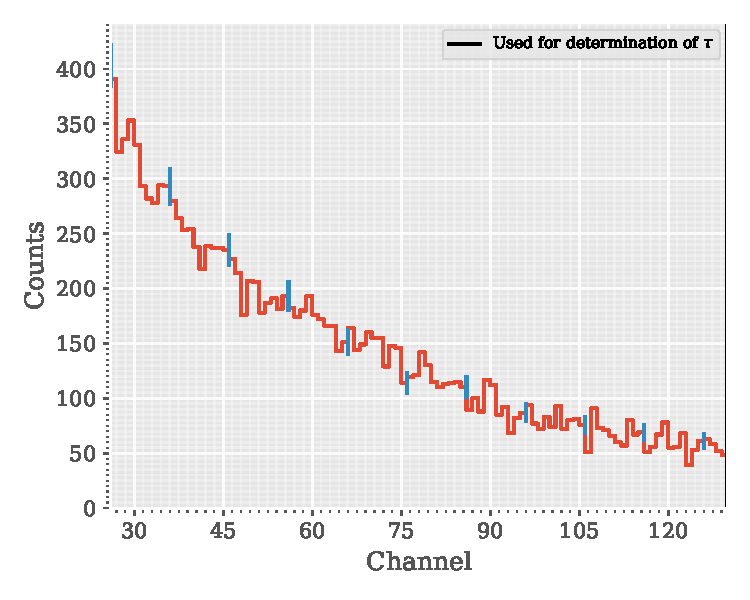
\includegraphics[width=0.5\linewidth]{spectrum_used.pdf}
    \caption{Analyzed part of the Spectrum}
    \label{fig:spec_used}
\end{floatingfigure}
For the evaluation of the main experiment, only the channels 25 through to 130 were used, as the lower channels are significantly influenced by other decay processes, such as the captured decay of $\mu^-$ or protons created by the through-flying muons in the scintillator, and the higher channels have a significant error due to their low event counts (with the data being Poisson-distributed, the relative error can be calculated to be $\dfrac{1}{\sqrt{N}}$, which at the upper end of the analyzed spectrum comes to about 15\% error). This results in $T=4.375\mus$ \Cref{fig:spec_used} shows the analyzed data with occasional blue errorbars for orientation.
%For the sake of readability, in the following $\tau$ always means the already optimized parameter, i.e. $\hat{\tau}$
\subsubsection{Maximum Likelihood Method applied to the exponential decay law}\label{sec:evalexp}
As already discussed in the theoretical part, 
to determine the best value of $\tau$ in this model, one has to solve this transcendental equation:
\begin{equation}
    0 = \frac{1}{N}\sum_{k=1}^{K} N_kt_k + \frac{T\e^{-T/\hat{\tau}}}{1-\e^{-T/\hat{\tau}}} -\hat{\tau}. \label{eq:likexp}
\end{equation}
$t_k$ here is the time in the middle of the interval, as that is estimated to be the average time at which events in this bin occur.\\
To achieve this numerically, \verb+scipy.optimize.fsolve+ was used, with an initial guess of $\tau_0=2\mus$. \verb+fsolve+ uses \textsc{Minipack}'s \say{hybrd}-algorithm for this task. Within eight iterations, the result was determined down to machine precision to be 
\[
\hat{\tau}=2.19\mus.
\]
In \cref{fig:exp}, the situation is displayed graphically.
\textbf{Error-calculation}
To estimate the error, one can use Gaussian error propagation, as the result is achieved analytically (save for the numeric solution of the final equation, but this error is negligible). In differentiating \cref{eq:likexp}, one has to use implicit differentiation (i.e. \[f^\prime (x)=-\dfrac{{\partial F(x, f(x))}/{\partial x}}{{\partial F(x, f(x))}/{\partial y}},
\]\begin{floatingfigure}{0.6\linewidth}
 \centering
    \includesvg[width=0.6\linewidth]{exp.svg}
    \caption{\cref{eq:likexp} around its root, with errorbars}
    \label{fig:exp}
\end{floatingfigure} where $x=N_k,\: f(x)=y=\hat{\tau}$ and $F(x, f(x))$ is \cref{eq:likexp}. The subscript denotes partial differentiation with respect to that variable.) The y-differentiation leads to a correction factor
\[
c = 1-\dfrac{T^2\mathrm{e}^\frac{T}{\tau}}{\hat{\tau}^2\left(\mathrm{e}^\frac{T}{\hat{\tau}}-1\right)^2} \approx 0.275
\]
by which the equation in \cite{anleitung} has to be divided.  The differentiation with respect to x leads to the form seen in \cite{anleitung}, but with an additional (however negligible) summand due to the fact that $N$ is dependent on $N_k$ (that is, $N=\sum_k^KN_k$). If one interprets N as a dependent parameter, one gets for its error:
\[
\Delta N = \sqrt{\sum_{k=1}^K\sqrt{N_k}^2} = \sqrt{N}.
\]
One can then calculate $\dfrac{\partial F}{\partial N}=-\dfrac{\sum_k^KN_kt_k}{N^2}$, getting the final equation
\[\Delta\hat{\tau}=\frac{1}{c\cdot N}\sqrt{\sum_{k=1}^KN_kt_k^2+\dfrac{\left(\sum_{k=1}^KN_kt_k\right)^2}{N^3}}=0.06\mus.
\]
\clearpage
\subsubsection{Application of the max-log likelihood method to a Poisson distribution}
\begin{floatingfigure}{0.6\linewidth}
 \centering
    \includesvg[width=0.55\linewidth]{pois.svg}
    \caption{The relevant part of the modified likelihood-function around its minimum.}
    \label{fig:pois}
\end{floatingfigure}
We now use the probability to measure $N_k$ events in an interval $(t_k, t_k+\Delta t)$, which is described by a Poisson-distribution $P(N_i|f_i)=\dfrac{f_i^{N_i}\cdot\e^{-f_i}}{N_i!}$ around an expected value 
\begin{align}
f_i&\approx\frac{N_0}{\tau}\e^{-(t_i+\Delta t/2)/\tau}\cdot\Delta t, \label{eq:fi}\\
N_0&=\frac{N}{\e^{t_1/\tau}-\e^{-(t_K+\Delta t)/\tau}},
\end{align}
where $N$ is the total number of events. Here, the starting time is irrelevant, as will become clear further below. \\
One can simplify finding the maximum of the likelihood-function, so that one only has to find the minimum of
\[
2\sum_iN_i\ln f_i,
\]
which is done with the help of \verb+scipy.optimize.minimize+. \verb+minimize+ uses the L-BFGS-B method for this, within the given bounds of (1\mus,3\mus) and terminated successfully within 15 iterations at
\[
\hat{\tau}=2.191\mus.
\]
This result is before rounding the exact same as the one achieved in the previous section down to the seventh decimal place, which is more than should be expected for two different methods. \\
Indeed, if one expands the $\ln f_i$-term, one finds that:
\[
\ln f_i = \mathrm{const.}-\ln\left(1-\e^{-T/\tau}\right)-\ln(\tau)-\frac{\overbrace{t_i-t_1+\Delta t/2}^{\text{Channel-centers from 0}}}{\tau}
\]
If one now compares 
\[
\sum_i(N_i\ln f_i)=\sum_iN_i\cdot\left(\mathrm{const.}-\ln\left(1-\e^{-T/\tau}\right)-\ln(\tau)-\frac{t_i-t_1+\Delta t/2}{\tau}\right)
\]
with \cref{eq:Lexp}, one can see that these are, barring a constant, the same equations and their minimizing should yield the same value.
\paragraph{Error-calculation}
By multiplying with -2, one can take the error of the estimate by taking the width of the curve one unit above the minimum, which gives:
\begin{gather}
    \Delta \hat{\tau} = 0.034 \mus.
\end{gather}
The situation is presented in \cref{fig:pois}.
\clearpage
\subsubsection{Application of the max-log likelihood method to a Gauss-distribution}
\begin{floatingfigure}{0.5\linewidth}
 \centering
    \includesvg[width=0.5\linewidth]{gauss.svg}
    \caption{The $\chi^2$-function around its minimum.}
    \label{fig:gauss}
\end{floatingfigure}
The idea here is the same as in the previous section, however, one assumes an underlying Gauss-distribution \[P(N_i|\tau)=\dfrac{1}{\sqrt{2\pi\sigma_i^2}}\exp{(-\dfrac{N_i-f_i)^2}{2\sigma_i^2}}.\] $f_i$ is the same as in \cref{eq:fi}, $\sigma$ is estimated to be $\sqrt{N_i}$. In this case, only 
\[
\chi^2=\sum_i\frac{(N_i-f_i)^2}{\sigma_i^2}
\]
has to be minimized, in the same way as above, this time taking 13 iterations to yield
\[
\hat{\tau}=2.201\mus.
\]

The $\chi^2$ value there is 144.6. At 104 channels and thus 103 degrees of freedom, this means that the $\chi^2$-test is passed. The error can be calculated as above to be 
\[
\Delta \hat{\tau} = 0.034\mus.
\]
The situation is illustrated in \cref{fig:gauss}.
\paragraph{Calculating the Fermi coupling constant $G_F$ and $v$}
In order to calculate the the Fermi coupling constant, one uses \cref{eq:fermi}
\begin{equation}
    \tau^{-1} = G_F^2\cdot \frac{m_{\mu}^5}{196\pi} \Longleftrightarrow G_F = \left(196\pi \tau^{-1}m_{\mu}^{-5} \right)^{\frac{1}{2}}
\end{equation}
For the vacuum expectation value $v$ of the \textsc{Brout-Engert-Higgs}-field one uses the weak coupling constant \cite{anleitung} and \cref{eq:higgs}:
\begin{equation}
    \sqrt{2}G_F=\frac{1}{v^2} \Longleftrightarrow v=\left ( \frac{1}{\sqrt{2}G_F}\right)^{\frac{1}{2}}
\end{equation}
\begin{table}[!htp]
    \centering
        \caption{Different $G_F$, $\tau$, and $v$ values for different methods where the Maximum Likelihood Method has been applied to. Literature values from \cite{literatur}\cite{Zyla:2020zbs}\cite{higgs}.}
    \begin{tabular}{c||c|c|c|c}
         &\textbf{Exp. decay}&\textbf{Poisson distr.}&\textbf{Gaussian distr.} &\textbf{Literature}\\\hline \hline
         $\tau \,/\, \mus$&2.19&2.191&2.201&2.19703\\ \hline
         $G_F \,/ \, \num{e-5}\si{\per\giga\eV\squared}$&1.165& 1.165& 1.163&1.166 3787\\ \hline
         $v \,/ \, \si{\giga \eV}$&246.3&246.3&246.6&246.8\\ \hline
         $\Delta \tau \,/\, \mus$&0.06&0.034&0.034&0.00004 \\ \hline
         $\Delta G_F / \num{e-8}\si{\per\giga\eV\squared}$&1.6& 0.9 &0.9&0.0000006 \\ \hline
         $\Delta v \,/ \, \si{\giga \eV}$&1.7& 1.0 & 1.0&0.0015
    \end{tabular}
    \label{tab:results}
\end{table}
For the computation of the errors $\Delta G_F$ and $\Delta v$, gaussian error propagation is used as follows, while for the muon mass, the literature value in natural units with neglectible uncertainty $m_{\mu}=\SI{109.6583745}{\mega \eV}$ is used \cite{literatur}:
\begin{align}
    \Delta G_F =& \frac{1}{2}\cdot \sqrt{\frac{192\pi^3}{m_{\mu}^5\cdot \tau^3}} \cdot \Delta \tau \\
    \Delta v =& \frac{1}{2^{\frac{5}{4}}\cdot G_F^{\frac{3}{2}}} \cdot \Delta G_F
\end{align}
\section{Discussion}
The measurement time for this experiment was $t=\SI{513808}{\second}$ with a total of \\$N=55338$ events. This means that events were measured with a rate of $0.108\,\si{\per\second}$, and that therefore there were likely only very few events lost due to happening in the interval occupied by other decays.\\\\
The values found for $\tau$ fit well with the literature-value of \[\tau=\SI{2.19703\pm0.00004e-6}{s} \cite{Zyla:2020zbs},\] which is well within their statistical error. The first and second methods of determining $\tau$ are mathematically identical, as such, presenting them as two different results with different uncertainties is debatable. Here, it is being justified as illustrating the difference between the two methods and the influence of rounding. The analysis based on a Gauss-distribution fits well with the other results, as the Gauss-distribution is a limit of the Poisson-distribution for a large large expectation value (here $f_i$), which is given in this experiment. That it returns a bigger result is not surprising, as the Poisson-distribution falls steeper toward smaller values. \\
It has to be noted that changing the analyzed channels influences the result quite dramatically, which reflects the large amount of noise from different processes, such as from captured muons, particles created by the through-flying muon or afterpulsing of the PMT. Save for the last effect however, they have a small time constant compared to the muon-decay and can thus be filtered out by discarding early channels, as done here. Longer measurement and more sophisticated analysis of the events would lower the statistical error by allowing more events to be measured.\\
The values for the Fermi constant $G_F$, \textsc{Brout-Engert-Higgs}-field expectation value $v$ nicely fit to the literature values, as can be seen in \cref{tab:results} with respect to their individual measurement uncertainties.


\printbibliography

\section{Appendix}
\subsection{Code}
Only the code used for data-analysis is given, with the values of the class variables commented in.
\begin{verbatim}
import numpy as np
from scipy.optimize import minimize_scalar
from scipy.optimize import fsolve


class LikelihoodFuncs:

    def __init__(self, n_i, t, T, tick=1 / 24):
        # N = N_channels[intervals[0]:intervals[1]]
        # t = np.arange(0, -intervals[0] + intervals[1]) * tick + tick / 2
        # T = t[-1] + tick - t[0]
        self.n_i = n_i
        self.t = t
        self.T = T
        self.N = np.sum(n_i)
        self.tick = tick

    def exponential(self, x):
        """Returns the function to be solved for Maximum-Likelihood 
        using the exponential decay model"""
        return (1 / self.N * np.sum(self.n_i * self.t) + (self.T * 
        np.exp(-self.T / x) / (1 - np.exp(-self.T / x))) - x)

    def pois(self, x):
        """Returns the relevant part of log(L) to be minimized 
        for Poisson-distributed data"""
        try:
            1 / x
        except ZeroDivisionError:
            return
        # As defined in the instructions
        N0 = self.N / (np.exp(-self.t[0] / x) - np.exp(-(self.t[-1] + 
        self.tick) / x))
        f_i = N0 / x * np.exp(-(self.t + self.tick/2) / x) * self.tick
        return 2 * np.sum(-self.n_i * np.log(f_i))

    def gauss(self, x):
        """Returns chi^2 to be minimized for Gauss-distributed data"""
        try:
            1 / x
        except ZeroDivisionError:
            return
        # As in instructions
        N0 = np.sum(self.n_i) / (np.exp(-self.t[0] / x) - np.exp(-(self.t[-1]
        + self.tick) / x))
        f_i = N0 / x * np.exp(-(self.t + self.tick/2) / x) * self.tick
        return np.sum((self.n_i - f_i) ** 2 / f_i)

    def L_exp(self, width, step=1000, guess=2):
        """
        Gives back root of expression as well as value-array of expression
        in width/2 around the root
        :float guess: initial guess of root
        :float width: plotting width
        """
        Nt = np.sum(self.n_i * self.t)
        # find \hat{\tau} as the root of the function
        tau = fsolve(self.exponential, guess, xtol=0, full_output=True)  
        tau = tau[0]
        # correcting factor for the error calculation
        correction = (self.T ** 2 * np.exp(self.T / tau)) / (tau ** 2 *
        (np.exp(self.T / tau) - 1) ** 2) - 1
        # Error-calculation
        sigma_tau = abs(1 / (self.N * correction) * 
        np.sqrt(np.sum(self.n_i * self.t ** 2) 
        + 1 / self.N ** 3 * Nt ** 2))
        # x-array for plot
        support = np.linspace(tau - width / 2, tau + width / 2, step)  
        L_exp_x = [self.exponential(xi) for xi in support]  # y-data for plot
        return (sigma_tau, self.exponential(tau), tau), (support, L_exp_x), False

    def minimize(self, func, width, step=100, limits=(1, 3)):
        """
         Gives back minimum, standard deviation from minimum of func as well as 
         value-array of func over width
         func: function to be minimized
         width: width of the plot
         step: how many support points should be created
         limits: range in which the minimum should be found
        """
        tau = minimize_scalar(func, limits)
        tau_x = tau.x

        def find_sigma():
            """
            Finds the x-distance from the minimum on the curve if y-value is raised
            by 1 unit, thereby finding the standard deviation
            """
            return (np.abs(tau_x - fsolve(lambda x: func(x) - 
            func(tau_x) - 1, tau_x - 1)),
            np.abs(tau_x - fsolve(lambda x: func(x) - 
            func(tau_x) - 1, tau_x + 1)))

        # Same as in L_exp
        support = np.linspace(tau_x - width / 2, tau_x + width / 2, step)
        L_plot_y = [func(xi) for xi in support]
        return (find_sigma(), func(tau_x), tau_x), (support,
        L_plot_y), True
\end{verbatim}
\end{document}
